\documentclass{article}

% if you need to pass options to natbib, use, e.g.:
% \PassOptionsToPackage{numbers, compress}{natbib}
% before loading nips_2016
%
% to avoid loading the natbib package, add option nonatbib:
% \usepackage[nonatbib]{nips_2016}

\usepackage[final]{nips_2016}
\usepackage{graphicx}
\usepackage{placeins}
\usepackage{subcaption}

% to compile a camera-ready version, add the [final] option, e.g.:
% \usepackage[final]{nips_2016}

\usepackage[utf8]{inputenc} % allow utf-8 input
\usepackage[T1]{fontenc}    % use 8-bit T1 fonts
\usepackage{hyperref}       % hyperlinks
\usepackage{url}            % simple URL typesetting
\usepackage{booktabs}       % professional-quality tables
\usepackage{amsfonts}       % blackboard math symbols
\usepackage{nicefrac}       % compact symbols for 1/2, etc.
\usepackage{microtype}      % microtypography

\title{Topical classification of comments in MOOC discussion forums}

% The \author macro works with any number of authors. There are two
% commands used to separate the names and addresses of multiple
% authors: \And and \AND.
%
% Using \And between authors leaves it to LaTeX to determine where to
% break the lines. Using \AND forces a line break at that point. So,
% if LaTeX puts 3 of 4 authors names on the first line, and the last
% on the second line, try using \AND instead of \And before the third
% author name.

\author{
  Bita Akram, Devarshi Pratap Singh, Pranjal Deka, Simerdeep Singh Jolly \\
  Department of Computer Science\\
  North Carolina State University\\
  Raleigh, NC 27606 \\
  \texttt{\{bakram,dsingh4,pdeka,sjolly\}@ncsu.edu} \\
  %% examples of more authors
  %%\And
  %%Coauthor \\
  %%Affiliation \\
  %%Address \\
  %%\texttt{email} \\
  %%\AND
  %%Coauthor \\
  %%Affiliation \\
  %%Address \\
  %%\texttt{email} \\
  %% \And
  %% Coauthor \\
  %% Affiliation \\
  %% Address \\
  %% \texttt{email} \\
  %% \And
  %% Coauthor \\
  %% Affiliation \\
  %% Address \\
  %% \texttt{email} \\
}

\begin{document}
% \nipsfinalcopy is no longer used

\maketitle

\begin{abstract}
MOOCs provide ample opportunities for facilitating education among a large group of learners. Hence, careful analysis of trace data obtained from interactions of learners with online courses can lead to an efficient and useful implementation of MOOCs. In this project we use Naive Bayes and a variety of SVM classification methods to topically classify comments in MOOCs' discussion forums for a k-12 teacher professional development class. The results of our study shows an advantage of utilizing linear SVM, and a disadvantage of using sigmoid SVM over other SVM approaches in classifying MOOCs comments.
\end{abstract}

\section{Introduction and Background}

With the emergence of technology and more specifically Internet, a new era in education is beginning. Taking advantage of accessibility and tremendous resources available on the Internet, open online courses are becoming more and more prevalent. Despite the great opportunity that massive open online courses (MOOCs) provide for learners, many issues arise by the autonomous nature of MOOCs and the lack of social interactions compared to the conventional classrooms. One of the main tools for interaction among learners are discussion forums. Hence, forums are a rich resource for evaluating students’ progress, satisfaction and learning. In this project, we aim to classify forum discussions based on their categorical types such as questioning, reflections, scaffolding, and also levels of critical thinking such as not applicable, undeveloped thinking, and critical thinking.

To aim for this purpose, we first conduct feature extraction using bag of words. Since the coding scheme uses certain words to distinguish between different topics, bag of words seems like a suitable candidate to classify between different topics. On the other hand bag of words produce a large number of features, many of which might not be deterministic of the type of our project. Hence, we reduce the dimension of our features using PCA, to capture the significant variations in our data-set. Next, we apply a couple of different classification methods including Naive Bayes and SVM and compare them through cross-validation to pick the best classification approach. Naive Bayes classification method is a fast and easy method to apply. However, having high dimensions SVM might be able to provide more accurate results and less overfitting.

\section{Related Work}
Many studies have attempted to understand students' interactions with MOOCs through pattern recognition and data-mining. For example, a study demonstrated in [7] used trace-data to build behavior patterns of low and high achieving students. In another study [8], the relevance of the course threads are ranked using linear regression and generative models.

In this study we are going to classify forum discussions based on their content. Past studies like [10] have shown that supervised models perform better when clustering short noisy data. We hence plan to use supervised models trained on hand-coded forum discussions. An unsupervised clustering method, k-medoids with greedy seed selection approach, is used to cluster discussion forum comments based on their content in one study [6]. In this study we apply Naive Bayes and SVM to classify the discussion forum comments. SVM has also been used for sentiment analysis in [9], which combines data from multiple resources through unigram models to produce more accurate results.

\section{Proposed Method}

In this section, we describe our approach of classifying topic category based on discussion text of MOOC discussion forums. Our dataset [4] consists of 487 samples of conversation data in a MOOC discussion forum. In particular, it consists of comments shared between learners in the forum and other attributes like timestamp of comment, title of discussion, category of discussion, type of comment (eg. question, statement, reflection etc) and level of critical thinking the comment represents. We predicted the discussion category based on the comment text in the forum.

\subsection{Data Cleaning}

We cleaned the dataset to render it free from all HTML tags. We then created a training dataset that contained the Comment Text and Discussion Category attributes. We further removed those  Discussion Category attributes that contained less than 10 samples. This left us with 5 Discussion Categories containing 399 training samples of Comment Text.

\subsection{Feature Extraction and Dimension Reduction}

We used a bag of words approach to perform feature extraction of all words in our dataset. For the 399 samples in our dataset and using document frequency as our feature parameter, we extracted 4023 features. This was represented in the form of a matrix having 399 rows and 4023 columns, each element representing the weight of a feature. We used the CountVectorizer in Python to extract the features. Next we performed dimension reduction using PCA to reduce the dimensions of our feature vector. We observed that 31 features had their standard deviation above 1, hence we reduced our dimensions from 4023 to 31. The plot of our PCA analysis is shown in Figure 1.


\begin{figure}[h!]
  \centering
  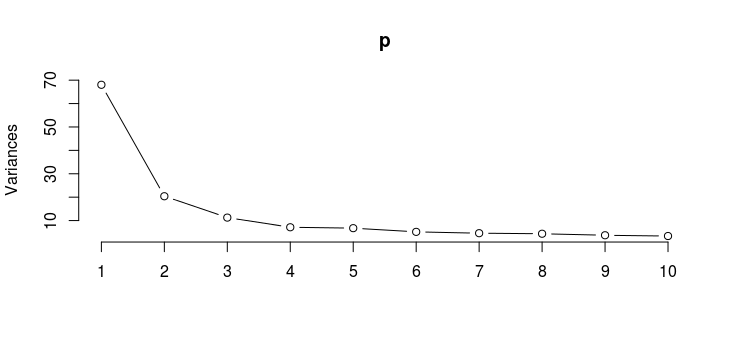
\includegraphics[width=90mm]{./images/pcaVariance.png}
  \caption{PCA variance plot.}
\end{figure}


\section{Experiments and Results}
\label{experiments_results}

After the preprocessing steps carried out on the dataset, we divided our dataset randomly into training set and testing set with a ratio of 70\% in training set and 30\% in testing set. Next we applied the SVM technique tuned on the best set of cost and gamma values and used it on 5 kernel types namely polynomial, radial basic function (gaussian kernel), sigmoid and quadratic. 

We deduced the confusion matrices of all techniques listed above for 5 label classes. From the confusion matrices depicted in Figures 2(a) to 2(d), we deduced the accuracy, precision and recall corresponding to each technique for our 5 target classes A to E. Our 5 target classes are decoded into their actual labels in Table 2. 

\begin{figure}[h!]
    \begin{subfigure}{0.5\textwidth}
      \centering
      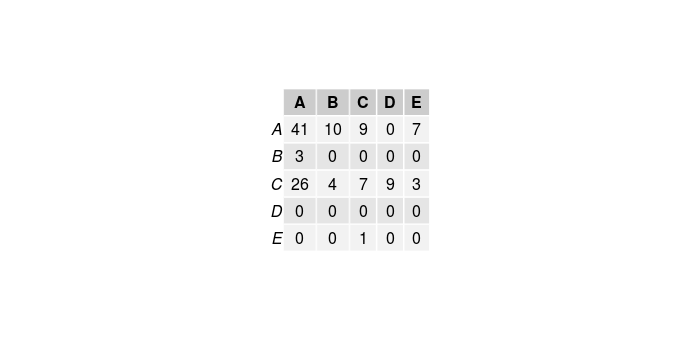
\includegraphics[width=110mm]{./images/CM_NB_Final.png}
      \caption{Confusion Matrix of Naive Bayes}
    \end{subfigure}
    \begin{subfigure}{.5\textwidth}
      \centering
      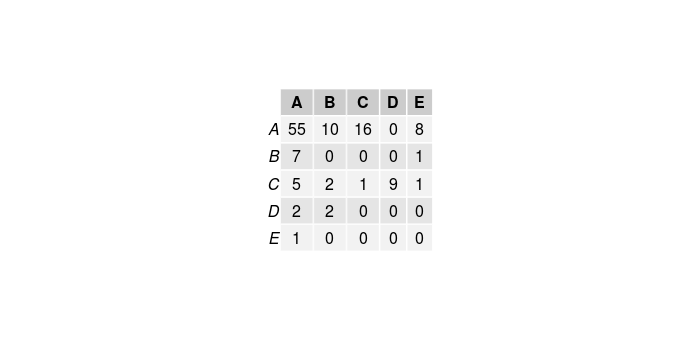
\includegraphics[width=110mm]{./images/CM_Linear_Final.png}
      \caption{Confusion Matrix of Linear SVM}
    \end{subfigure}

    \begin{subfigure}{.5\textwidth}
      \centering
      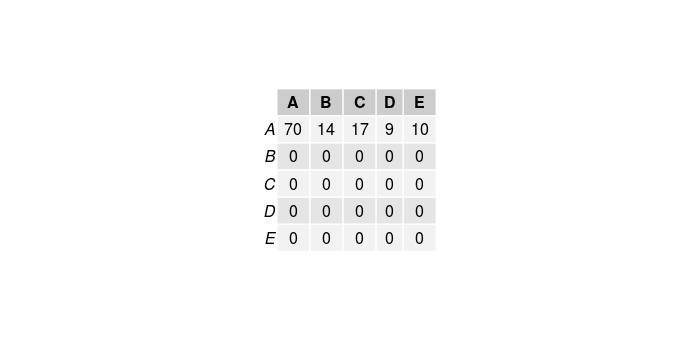
\includegraphics[width=110mm]{./images/CM_Quadratic_Final.png}
      \caption{Confusion Matrix of Polynomial, Quadratic and Radial SVM}
    \end{subfigure}
    \begin{subfigure}{.5\textwidth}
      \centering
      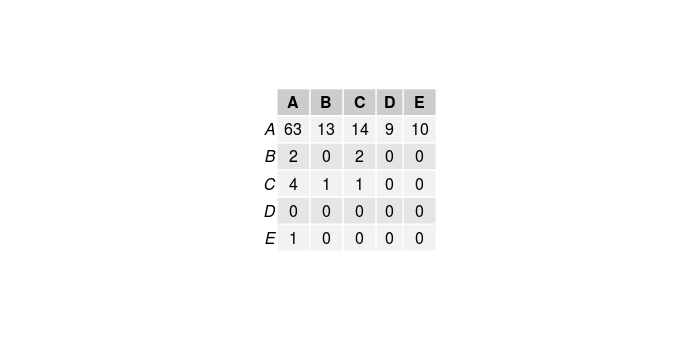
\includegraphics[width=110mm]{./images/CM_Sigmoid_Final.png}
      \caption{Confusion Matrix of Sigmoid SVM}
    \end{subfigure}
    \caption{Confusion matrices of various classification techniques}
\end{figure}

The overall accuracy of each of the techniques is shown in Table 1. 

\begin{table}[h!]
\caption{Overall Accuracy of Techniques}
  \label{table1}
  \centering
  \begin{tabular}{lll}
    \toprule
    \cmidrule{1-2}
    Method          & Accuracy             \\
    \midrule
    Naive Bayes     & $\sim$$40.00\%$      \\
    Linear SVM      & $\sim$$58.33\%$      \\
    Polynomial SVM  & $\sim$$58.33\%$      \\
    Radial SVM      & $\sim$$58.33\%$      \\
    Sigmoid SVM     & $\sim$$53.33\%$      \\
    Quadratic SVM   & $\sim$$58.33\%$      \\
    \bottomrule
  \end{tabular}
\end{table}

\begin{table}[h!]
\caption{Target Class Labels}
  \label{table1}
  \centering
  \begin{tabular}{lll}
    \toprule
    \cmidrule{1-2}
    Class Label     & Actual Class Value in Dataset            \\
    \midrule
    A     & Changes in what, how, when and where students learn?      \\
    B      & Major challenges to making recommended changes?      \\
    C  & Most important changes needed in K-12 education?       \\
    D     & Providing the technology tools (Technology \& Infrastructure and Budget \& Resources planning elements)      \\
    E     & Teacher and Administrator Preparedness      \\
    \bottomrule
  \end{tabular}
\end{table}

\FloatBarrier
\subsection{Techniques to be applied in future}

In future, we will be using the following classifiers on the input dataset to train and test the various models

\begin{itemize}
\item Decision Tree
\item Linear Regression
\item Logistic Regression
\item Max Entropy
\end{itemize}



\section*{Conclusion}
We used Naive Bayes as our baseline, which generated 40.00 \% accuracy in its overall classification. The results of applying different SVM demonstrated similar performance for linear, polynomial, radial and quadratic SVM with 58.33\% overall accuracy. Sigmoid SVM on the other hand showed less accurate results, 53.33\%, compared to the other SVM techniques. 

We further observed that the class accuracy of class A was highest $($$\sim$$53.3\%$$)$ for Polynomial, Radial and Quadratic SVM techniques. The precision of class A was highest $($$\sim$$90\%$$)$ for Sigmoidal SVM technique. The recall of class A was highest $($$\sim$$61.8\%$$)$ for Linear SVM technique. 

Going forward, in future we aim to improve the accuracy of our model by exploring other classification techniques like Decision Tree, Max Entropy, Linear and Logistic Regression. We wish to improve our feature extracted matrix by accounting for ngram features. We also plan to use LDA (Linear Discriminant Analyzer) instead of PCA to improve our reduced feature space. We also aim to employ remaining dataset features in our analysis to improve the efficiency of classification technique. Furthermore we wish to apply k-fold cross validation to assess the accuracy of our model in a more rigorous manner.

\section*{References}   

\small

[1] Kellogg, Shaun, Sherry Booth, and Kevin Oliver. "A social network perspective on peer supported learning in MOOCs for educators." The International Review of Research in Open and Distributed Learning 15.5 (2014).

[2] Zadeh, Reza Bosagh, and Ashish Goel. "Dimension independent similarity computation." Journal of Machine Learning Research 14.1 (2013): 1605-1626.

[3] Ezen-Can, Aysu, et al. "Unsupervised modeling for understanding MOOC discussion forums: a learning analytics approach." Proceedings of the fifth international conference on learning analytics and knowledge. ACM, 2015.

[4] Kellogg, Shaun; Edelmann, Achim, 2015, "Massively Open Online Course for Educators (MOOC-Ed) network dataset",doi:10.7910/DVN/ZZH3UB, Harvard Dataverse, V1

[5] FAQ of SVM in R and Matlab http://www.csie.ntu.edu.tw/~cjlin/libsvm/faq.html

[6] Ezen-Can, Aysu, et al. "Unsupervised modeling for understanding MOOC discussion forums: a learning analytics approach." Proceedings of the fifth international conference on learning analytics and knowledge. ACM, (2015).

[7] Brinton, Christopher G., et al. "Learning about social learning in MOOCs: From statistical analysis to generative model." IEEE transactions on Learning Technologies 7.4 (2014): 346-359.

[8] Anderson, Ashton, et al. "Engaging with massive online courses." Proceedings of the 23rd international conference on World wide web. ACM, (2014).

[9] Mullen, Tony, and Nigel Collier. "Sentiment Analysis using Support Vector Machines with Diverse Information Sources." EMNLP. Vol. 4. 2004.

[10] Rosa, Kevin Dela, et al. "Topical clustering of tweets." Proceedings of the ACM SIGIR: SWSM (2011).

\section*{Appendix}

In our first proposal we proposed exploiting efficient data mining techniques to predict categories (eg. social, judicial, political, personal, health, sports) of tweets on Twitter. 
However, we changed the direction of our project to conduct topical classification on comments obtained from discussion forums in MOOCs. In this project we aim to topically cluster discussions obtained from forums of a K-12 teacher development online course. To aim for this purpose we use a data-set that has been hand-coded based on discussion contents. We train our classifier based on different approaches such as SVM and Naive Bayes models. We then compared the results of applying different techniques on our data-set to find the one that produces the highest accuracy.

The new proposal can be found here:
\url{https://github.com/simerdeep92/AldaProject/blob/master/documents/Proposal.pdf}

\subsubsection*{Divison of work}
Bita - Implement Decision Tree classifier and report accuracy. Explore remaining dataset attributes to improve efficiency of our model.\\
Devarshi - Implement Logistic Regression classifier and report accuracy. Apply ngram technique to feature extraction. \\
Pranjal - Implement Linear Regression classifier and report accuracy. Apply LDA to reduce dimensions.\\
Simerdeep - Implement Max Entropy classifier and report accuracy. Apply k-fold cross validation.


\end{document}

